% ----------------------------------------
% Documentation for JSLAB
% ----------------------------------------
\documentclass[12pt,a4paper]{article}
\usepackage{tabularx}
\usepackage{geometry}
\usepackage{listings}
\usepackage{fancyhdr}
\usepackage{lastpage}
\usepackage{tikz}
\usepackage{xcolor}
\usepackage{booktabs}
\usepackage{caption}
\usepackage{hyperref}
\usepackage{float}
\usepackage{varwidth}
\usepackage[most]{tcolorbox}

% Define variables
\newcommand{\yearvar}{$JSLAB_PUBLISH_YEAR$}
\newcommand{\appversion}{$JSLAB_APP_VERSION$}

% Colors
\definecolor{jsl-blue}{cmyk}{1,1,0,0}
\definecolor{jsl-orage}{cmyk}{0,.5,1,0}
\definecolor{jsl-green}{cmyk}{1,0,1,0.5}
\definecolor{jsl-gray}{cmyk}{0,0,0,0.5}
\definecolor{jsl-light-gray}{cmyk}{0,0,0,0.1}
\definecolor{jsl-yellow}{RGB}{247,223,30}

% Code
\lstdefinelanguage{JavaScript}{
  morekeywords=[1]{break, continue, delete, else, for, function, if, in,
    new, return, this, typeof, var, void, while, with},
  % Literals, primitive types, and reference types.
  morekeywords=[2]{false, null, true, boolean, number, undefined,
    Array, Boolean, Date, Math, Number, String, Object},
  % Built-ins.
  morekeywords=[3]{eval, parseInt, parseFloat, escape, unescape},
  sensitive,
  morecomment=[s]{/*}{*/},
  morecomment=[l]//,
  morecomment=[s]{/**}{*/}, % JavaDoc style comments
  morestring=[b]',
  morestring=[b]"
}[keywords, comments, strings]

\lstdefinestyle{JavaScriptStyle}{
    language=JavaScript,
    basicstyle=\fontfamily{pcr}\selectfont\footnotesize, 
    commentstyle=\color{jsl-green},
    keywordstyle=\bf\color{jsl-blue},
    stringstyle=\color{jsl-gray},
    breaklines=true,
    showstringspaces=false,
    captionpos=b,
    numbers=left,
    numberstyle=\tiny\color{gray},
    stepnumber=1,
    numbersep=10pt,
    inputencoding=utf8,
    extendedchars=true,
    literate=
        {°}{{\textdegree}}1
        {º}{{\textordmasculine}}1 
        {š}{{\v{s}}}1
        {Š}{{\v{S}}}1
        {č}{{\v{c}}}1
        {Č}{{\v{C}}}1
        {ž}{{\v{z}}}1
        {Ž}{{\v{Z}}}1
        {ć}{{\'{c}}}1
        {Ć}{{\'{C}}}1
        {θ}{{$\theta$}}1
        {µ}{{$\micro$}}1 
}

\newtcbox{\code}[1][]{%
    on line,
    colback=jsl-light-gray,
    colframe=jsl-light-gray, 
    boxrule=0pt, 
    arc=3pt,
    left=2pt,
    right=2pt,
    top=2pt,
    bottom=2pt,
    box align=base,
    fontupper=\ttfamily,
    #1
}

\newtcbox{\codeBlock}[1][]{%
    colback=jsl-light-gray,
    colframe=jsl-light-gray, 
    boxrule=0pt, 
    arc=3pt,
    left=2pt,
    right=2pt,
    top=2pt,
    bottom=2pt,
    box align=base,
    breakable,
    enhanced jigsaw,
    varwidth upper,
    fontupper=\ttfamily,
    #1
}

% Formating
\delimitershortfall=-1pt
\tolerance=1
\emergencystretch=\maxdimen
\hyphenpenalty=10000
\hbadness=10000

% Paper
\geometry{
  paperheight=297mm,
  paperwidth=210mm,
  top=40mm,
  bottom=22mm,
  right=20mm,
  left=25mm,
  headheight=45mm,
  headsep = 10mm,
}

\newcommand{\companyLogo}[2][1]{%
\begin{tikzpicture}[y=1cm, x=1cm, yscale=#1, xscale=#1, every node/.append style={scale=#1}, inner sep=0pt, outer sep=0pt]
  \path[fill=#2,line cap=butt,line join=miter,line width=0.1cm,shift={(0,2.3814000000000006)},scale=0.2646] (48.3133, 7.2898).. controls (48.3133, 7.2898) and (45.5748, 7.2298) .. (42.8363, 7.2385).. controls (42.5511, 7.2394) and (42.2572, 7.2395) .. (41.9563, 7.2387).. controls (37.4414, 7.2255) and (31.3175, 7.1544) .. (28.0006, 6.1414).. controls (21.9344, 4.2889) and (18.5966, 1.6908) .. (15.8504, -1.3797).. controls (15.3536, -1.9429) and (14.706, -2.7974) .. (13.9723, -3.8922).. controls (14.3648, -4.7541) and (14.5615, -5.7655) .. (14.5615, -6.9275).. controls (14.5615, -8.2166) and (14.3276, -9.3004) .. (13.8598, -10.1789).. controls (13.3919, -11.0574) and (12.795, -11.7496) .. (12.0693, -12.2557).. controls (11.3532, -12.7522) and (10.6227, -13.0816) .. (9.8779, -13.2439).. controls (9.5808, -13.3028) and (9.2396, -13.352) .. (8.8643, -13.3936).. controls (7.5711, -16.3864) and (6.3915, -19.737) .. (5.5781, -23.2604) -- (44.9074, -23.2898).. controls (45.292, -19.8927) and (45.6146, -16.9976) .. (45.9133, -14.2994).. controls (45.4314, -13.1253) and (45.19, -11.7645) .. (45.19, -10.2162).. controls (45.19, -7.5942) and (45.8113, -5.5113) .. (47.0529, -3.9666).. controls (47.4282, -0.5661) and (47.8187, 2.9505) .. (48.3133, 7.2898) -- cycle(53.9496, -2.5064).. controls (51.9444, -2.5064) and (50.3266, -3.1673) .. (49.0961, -4.4889).. controls (47.8656, -5.804) and (47.2504, -7.6529) .. (47.2504, -10.0357).. controls (47.2504, -12.2883) and (47.8624, -14.0657) .. (49.0863, -15.3678).. controls (50.3103, -16.6633) and (51.8728, -17.3111) .. (53.7738, -17.3111).. controls (55.3103, -17.3111) and (56.5766, -16.9335) .. (57.5727, -16.1783).. controls (58.5753, -15.4166) and (59.2914, -14.2545) .. (59.7211, -12.692) -- (56.9184, -11.8033).. controls (56.6775, -12.8515) and (56.2803, -13.6197) .. (55.727, -14.108).. controls (55.1736, -14.5963) and (54.5128, -14.8404) .. (53.7445, -14.8404).. controls (52.7029, -14.8404) and (51.8565, -14.4563) .. (51.2055, -13.6881).. controls (50.5544, -12.9199) and (50.2289, -11.6308) .. (50.2289, -9.8209).. controls (50.2289, -8.1152) and (50.5577, -6.8814) .. (51.2152, -6.1197).. controls (51.8793, -5.358) and (52.7419, -4.9771) .. (53.8031, -4.9771).. controls (54.5714, -4.9771) and (55.2224, -5.192) .. (55.7563, -5.6217).. controls (56.2966, -6.0514) and (56.6514, -6.6373) .. (56.8207, -7.3795) -- (59.682, -6.6959).. controls (59.3565, -5.5501) and (58.8682, -4.6712) .. (58.2172, -4.0592).. controls (57.1234, -3.024) and (55.7009, -2.5064) .. (53.9496, -2.5064) -- cycle(1.4217, -2.7506) -- (1.4217, -17.067) -- (4.3123, -17.067) -- (4.3123, -11.6666) -- (6.1971, -11.6666).. controls (7.5057, -11.6666) and (8.505, -11.5982) .. (9.1951, -11.4615).. controls (9.7029, -11.3508) and (10.201, -11.1262) .. (10.6893, -10.7877).. controls (11.1841, -10.4426) and (11.591, -9.9706) .. (11.91, -9.3717).. controls (12.229, -8.7727) and (12.3885, -8.0338) .. (12.3885, -7.1549).. controls (12.3885, -6.0156) and (12.1118, -5.0878) .. (11.5584, -4.3717).. controls (11.005, -3.649) and (10.3182, -3.1803) .. (9.4979, -2.9654).. controls (8.964, -2.8222) and (7.8182, -2.7506) .. (6.0604, -2.7506) -- (1.4217, -2.7506) -- cycle(15.7908, -2.7506) -- (21.8748, -2.7506).. controls (23.4048, -2.7506) and (24.5148, -2.8808) .. (25.2049, -3.1412).. controls (25.9015, -3.3951) and (26.4581, -3.8508) .. (26.8748, -4.5084).. controls (27.2915, -5.1659) and (27.4998, -5.9179) .. (27.4998, -6.7643).. controls (27.4998, -7.8385) and (27.184, -8.7271) .. (26.5525, -9.4303).. controls (25.921, -10.1269) and (24.977, -10.5663) .. (23.7205, -10.7486).. controls (24.3455, -11.1132) and (24.8598, -11.5136) .. (25.2635, -11.9498).. controls (25.6736, -12.386) and (26.2238, -13.1607) .. (26.9139, -14.274) -- (28.6619, -17.067) -- (25.2049, -17.067) -- (23.115, -13.9518).. controls (22.3728, -12.8385) and (21.865, -12.1386) .. (21.5916, -11.8521).. controls (21.3182, -11.5592) and (21.0285, -11.3606) .. (20.7225, -11.2564).. controls (20.4165, -11.1458) and (19.9314, -11.0904) .. (19.2674, -11.0904) -- (18.6814, -11.0904) -- (18.6814, -17.067) -- (15.7908, -17.067) -- (15.7908, -2.7506) -- cycle(32.2953, -2.7506) -- (37.5785, -2.7506).. controls (38.7699, -2.7506) and (39.6781, -2.8417) .. (40.3031, -3.024).. controls (41.143, -3.2714) and (41.8624, -3.7109) .. (42.4613, -4.3424).. controls (43.0603, -4.9739) and (43.516, -5.7486) .. (43.8285, -6.6666).. controls (44.141, -7.5781) and (44.2973, -8.7044) .. (44.2973, -10.0455).. controls (44.2973, -11.2239) and (44.1508, -12.2395) .. (43.8578, -13.0924).. controls (43.4997, -14.134) and (42.9887, -14.9772) .. (42.3246, -15.6217).. controls (41.8233, -16.11) and (41.1462, -16.4908) .. (40.2934, -16.7643).. controls (39.6553, -16.9661) and (38.8025, -17.067) .. (37.7348, -17.067) -- (32.2953, -17.067) -- (32.2953, -2.7506) -- cycle(4.3123, -5.1725) -- (5.7088, -5.1725).. controls (6.7505, -5.1725) and (7.4438, -5.205) .. (7.7889, -5.2701).. controls (8.2576, -5.3548) and (8.645, -5.5663) .. (8.951, -5.9049).. controls (9.257, -6.2434) and (9.41, -6.6731) .. (9.41, -7.1939).. controls (9.41, -7.6171) and (9.2993, -7.9882) .. (9.0779, -8.3072).. controls (8.8631, -8.6262) and (8.5636, -8.8606) .. (8.1795, -9.0104).. controls (7.7954, -9.1601) and (7.0337, -9.235) .. (5.8943, -9.235) -- (4.3123, -9.235) -- (4.3123, -5.1725) -- cycle(18.6814, -5.1725) -- (18.6814, -8.8053) -- (20.8201, -8.8053).. controls (22.2068, -8.8053) and (23.0727, -8.7467) .. (23.4178, -8.6295).. controls (23.7628, -8.5123) and (24.033, -8.3105) .. (24.2283, -8.024).. controls (24.4236, -7.7376) and (24.5213, -7.3795) .. (24.5213, -6.9498).. controls (24.5213, -6.468) and (24.3911, -6.0807) .. (24.1307, -5.7877).. controls (23.8768, -5.4882) and (23.5154, -5.2994) .. (23.0467, -5.2213).. controls (22.8123, -5.1887) and (22.1092, -5.1725) .. (20.9373, -5.1725) -- (18.6814, -5.1725) -- cycle(35.1859, -5.1725) -- (35.1859, -14.6549) -- (37.3441, -14.6549).. controls (38.1514, -14.6549) and (38.7341, -14.6093) .. (39.0922, -14.5182).. controls (39.5609, -14.401) and (39.9483, -14.2024) .. (40.2543, -13.9225).. controls (40.5668, -13.6425) and (40.8207, -13.1835) .. (41.016, -12.5455).. controls (41.2113, -11.901) and (41.309, -11.0253) .. (41.309, -9.9186).. controls (41.309, -8.8118) and (41.2113, -7.9622) .. (41.016, -7.3697).. controls (40.8207, -6.7773) and (40.5473, -6.315) .. (40.1957, -5.983).. controls (39.8441, -5.651) and (39.3982, -5.4264) .. (38.8578, -5.3092).. controls (38.4542, -5.218) and (37.6632, -5.1725) .. (36.4848, -5.1725) -- (35.1859, -5.1725) -- cycle(27.5357, -9.7939) -- (31.1723, -9.7939) -- (31.1723, -11.6123) -- (27.5357, -11.6123) -- (27.5357, -9.7939) -- cycle;
\end{tikzpicture}
}

\newcommand{\jslabLogo}[2][1]{%
\begin{tikzpicture}[y=1cm, x=1cm, yscale=#1, xscale=#1, every node/.append style={scale=#1}, inner sep=0pt, outer sep=0pt]
  \path[fill=jsl-yellow,rounded corners=#2] (0.0, 0.0) rectangle (16.6688, -16.6688);
  \path[fill=black,line width=0.2278cm] (3.5007, -15.6898).. controls (4.6304, -15.6898) and (5.4048, -15.0885) .. (5.4048, -13.7675) -- (5.4048, -9.4127) -- (4.1293, -9.4127) -- (4.1293, -13.7493).. controls (4.1293, -14.387) and (3.8651, -14.551) .. (3.446, -14.551).. controls (3.0087, -14.551) and (2.8265, -14.2503) .. (2.6261, -13.895) -- (1.5875, -14.5237).. controls (1.8881, -15.1614) and (2.4803, -15.6898) .. (3.5007, -15.6898) -- cycle;
  \path[fill=black,line width=0.2278cm] (8.4203, -15.6898).. controls (9.632, -15.6898) and (10.534, -15.0612) .. (10.534, -13.9132).. controls (10.534, -12.8473) and (9.9236, -12.3736) .. (8.8394, -11.9089) -- (8.5206, -11.7723).. controls (7.9739, -11.5354) and (7.7371, -11.3805) .. (7.7371, -10.9979).. controls (7.7371, -10.6881) and (7.9739, -10.4513) .. (8.3475, -10.4513).. controls (8.7119, -10.4513) and (8.9487, -10.6061) .. (9.1674, -10.9979) -- (10.1604, -10.3602).. controls (9.7414, -9.6222) and (9.1583, -9.3398) .. (8.3475, -9.3398).. controls (7.2086, -9.3398) and (6.4798, -10.0686) .. (6.4798, -11.0252).. controls (6.4798, -12.0638) and (7.0902, -12.5558) .. (8.0104, -12.9475) -- (8.3292, -13.0842).. controls (8.9123, -13.3393) and (9.2585, -13.4942) .. (9.2585, -13.9315).. controls (9.2585, -14.2959) and (8.9214, -14.5601) .. (8.393, -14.5601).. controls (7.7644, -14.5601) and (7.4091, -14.2321) .. (7.1358, -13.7857) -- (6.0972, -14.387).. controls (6.4707, -15.1249) and (7.236, -15.6898) .. (8.4203, -15.6898) -- cycle;
  \path[fill=black,line width=0.2278cm] (11.527, -15.6078) -- (15.6085, -15.6078) -- (15.6085, -14.4872) -- (12.8025, -14.4872) -- (12.8025, -9.4127) -- (11.527, -9.4127) -- cycle;
\end{tikzpicture}
}

% Tabele
\newcolumntype{L}[1]{>{\raggedright\let\newline\\\arraybackslash\hspace{0pt}}m{#1}}
\newcolumntype{C}[1]{>{\centering\let\newline\\\arraybackslash\hspace{0pt}}m{#1}}
\newcolumntype{R}[1]{>{\raggedleft\let\newline\\\arraybackslash\hspace{0pt}}m{#1}}

\fancypagestyle{tekst}{
    \fancyhf{}
    \fancyhead[C]{
        \begin{minipage}{16.5cm}
            \begin{minipage}{2cm}
                \jslabLogo[0.1]{0.1cm}
                \vspace{1mm}
            \end{minipage}
            \begin{minipage}{2.6cm}
                \vspace{1mm}
                
                \companyLogo[0.15]{black}
            \end{minipage}
           \begin{minipage}{5cm}
                \footnotesize
                web: \href{https://pr-dc.com}{pr-dc.com} \\
                email: \href{mailto:info@pr-dc.com}{info@pr-dc.com}\\
                github: \href{https://github.com/PR-DC}{github.com/PR-DC}
            \end{minipage}  
           \begin{minipage}{6.5cm}
                \raggedleft {\large\textbf{JSLAB \appversion}} \\
                \raggedleft DOCUMENTATION
            \end{minipage}
            \vspace{-5mm}
        \end{minipage}
    }

    \fancyfoot[C]{\vspace{2mm} \bfseries {\thepage} / \pageref{LastPage}}
    \renewcommand{\headrulewidth}{0.4pt}
    \renewcommand{\headrule}{{\color{jsl-yellow}\hrule}}
    \renewcommand{\footrulewidth}{0.4pt}
    \renewcommand{\footrule}{{\color{jsl-yellow}\hrule}}

}

\makeatletter
\newcommand*{\ov}[1]{%
  $\m@th\overline{\mbox{#1}\raisebox{5mm}{}}$%
}

\renewcommand{\arraystretch}{1.2}
\renewcommand{\aboverulesep}{0}
\renewcommand{\belowrulesep}{0}

% Podesavanja naslova slika
\DeclareCaptionLabelSeparator{bar}{ - }
\captionsetup{labelsep=bar}

% ----------------------------------------
% POCETAK DOKUMENTA
% ----------------------------------------
\begin{document}

% ----------------------------------------
% NASLOVNA STRANA
% ----------------------------------------
\begin{titlepage}

    \centering
    
    \vphantom{vspace}
    
    \vspace{5mm}
    
    \companyLogo[0.5]{black}
	
    \vspace{5mm}
    
    \centerline{\footnotesize{web: \href{https://pr-dc.com}{pr-dc.com}, email: \href{mailto:info@pr-dc.com}{info@pr-dc.com}, github: \href{https://github.com/PR-DC}{github.com/PR-DC}}}
    
    \vspace{5mm}

    \hrule
	
    \vspace{10mm}

    \jslabLogo[0.2]{0.1cm}

    \vspace{8mm}
    
    {\Huge\textbf{JSLAB \appversion} \par}
   
    \vspace{2mm}

    {\LARGE DOCUMENTATION \par}

    \vspace{8mm}
    
   \href{https://github.com/PR-DC/JSLAB}{github.com/PR-DC/JSLAB}
    
    \vspace{8mm}
    
    \hrule
    
    \vfill
    
    \textbf{PRDC d.o.o.}, Novo naselje bb, 22310 Šimanovci, Republic of Serbia

\end{titlepage}

% ----------------------------------------
% Contents
% ----------------------------------------
\pagestyle{tekst}
\tableofcontents
\newpage

% ----------------------------------------
% Start of document
% ----------------------------------------

% --------------------
\section{About JSLAB}

Welcome to the \textbf{JSLAB} Documentation! This guide provides comprehensive information for users and contributors, detailing the features, usage, and contribution guidelines to ensure a consistent and high-quality codebase.

\begin{figure}[H]
    \centering
    \centerline{\jslabLogo[0.3]{0.2cm}}
    \caption{JSLAB logo}
    \label{fig:logo}
\end{figure}

The \textbf{JavaScript Laboratory (JSLAB)} is an open-source environment designed for scientific computing, data visualization, and various other computer operations. Inspired by \textit{GNU Octave} and \textit{Matlab}, \textbf{JSLAB} leverages the advantages of JavaScript, including its blazing speed, extensive examples, backing by some of the largest software companies globally, and the vast community of active programmers and software engineers.

\begin{figure}[H]
    \centering
    \includegraphics[width=0.8\textwidth]{resources/JSLAB_gui.png}
    \caption{JavaScript Laboratory (JSLAB) GUI}
    \label{fig:jslab}
\end{figure}

The program was developed to fulfill the need for performing calculations in a programming language that allows for code reuse in later project stages. JavaScript was chosen for its speed, dynamic nature, interpretability, extensive library support, large existing codebase, backing by major software companies, and the ability to create both desktop and mobile applications.

\textbf{JSLAB} offers a streamlined, dual-window interface designed to boost productivity and foster innovation. The main window combines a versatile workspace with a sandbox terminal, allowing users to run, test, and iterate on code in real time. The dedicated editor window introduces the \textbf{.JSL file format}—a plain text format tailored for \textbf{JSLAB} scripts. With advanced linting and intelligent autocompletion, the editor makes it easy to write precise, reusable code with minimal errors.

% ----------
\subsection{Why Choose JSLAB?}

\begin{itemize}
    \item \textbf{Backed by Leading Investments}

JavaScript is supported by major industry investments, ensuring continuous innovation and robust development. Our commitment to excellence makes \textbf{JSLAB} a trusted choice for professionals and organizations worldwide.

\item \textbf{Powered by JavaScript, Trusted by Giants}

Join the ranks of top companies who leverage JavaScript for their mission-critical applications. With \textbf{JSLAB}, you benefit from the same reliable and scalable technology that powers some of the most advanced projects on Earth and beyond.

\item \textbf{Thriving Community and Massive User Base}

Become part of a vibrant and growing community of JavaScript developter. Extensive support network and active forums ensure you always have the resources and assistance you need to succeed.

\item \textbf{Comprehensive Functionality Comparable to Leading Tools}

\textbf{JSLAB} bridges the gap between JavaScript and specialized scientific tools. Enjoy functionalities equivalent to MATLAB, GNU Octave, Python, R, and Julia, all within a single, unified platform. Perform data analysis, machine learning, numerical computations, and more with ease.

\item \textbf{Seamless and Native GUI with HTML, CSS, and SVG}

Design intuitive and visually appealing graphical user interfaces using native HTML, CSS, and SVG. Create interactive dashboards, custom visualizations, and responsive layouts without the need for additional frameworks.

\item \textbf{Extend with Native Modules via NPM and C++/C}

Enhance \textbf{JSLAB}’s capabilities by integrating native modules from npm, built with C++ and C. Tap into a vast ecosystem of extensions and customize your environment to meet your specific needs, ensuring maximum performance and flexibility.

\item \textbf{Join the JSLAB Revolution Today!}

Experience the seamless integration of powerful scientific computing and the flexibility of JavaScript. Whether you're developing complex algorithms, analyzing vast datasets, or creating innovative applications, \textbf{JSLAB} empowers you to achieve more.

\end{itemize}

% ----------
\subsection{License}
This program is free software: you can redistribute it and/or modify it under the terms of the GNU Lesser General Public License as published by the Free Software Foundation, either version 3 of the License, or (at your option) any later version.

This program is distributed in the hope that it will be useful, but WITHOUT ANY WARRANTY; without even the implied warranty of MERCHANTABILITY or FITNESS FOR A PARTICULAR PURPOSE. See the GNU Lesser General Public License for more details.

You should have received a copy of the GNU Lesser General Public License along with this program. If not, see \url{https://www.gnu.org/licenses/}.

\vspace{5mm}

Copyright (C) \yearvar\; PR-DC info@pr-dc.com

\vspace{8mm}

% --------------------
\section{About documentation}

This documentation serves as a comprehensive guide for both users and contributors of the \textbf{JSLAB} Library. It covers an introduction to the project, detailed features, installation and setup instructions, user interface overview, practical examples, coding standards, build instructions, contribution guidelines, and mechanisms for providing feedback.

The documentation is structured to provide clear and detailed information, ensuring that both new users and seasoned contributors can effectively utilize and contribute to the \textbf{JSLAB} project.

% --------------------
\section{Coding style}
\label{coding-style}

% ----------
\subsection{Documentation and Comments}

Clear documentation is essential for maintaining and understanding the codebase. We utilize JSDoc for structured documentation and inline comments to clarify complex logic.

\begin{itemize}
  \item \textbf{JSDoc:} Use JSDoc comments to document files, classes, methods, parameters, and return values.
  
  \item \textbf{Inline Comments:} Add comments to explain non-trivial code segments.
\end{itemize}

\begin{lstlisting}[style=JavaScriptStyle]
/**
* Constructs the JSLAB library environment.
* @param {Object} config Configuration options.
*/
constructor(config) {
  // Initialize properties
  this.config = config;
  // ... other initializations
}
\end{lstlisting}

% ----------
\subsection{Naming Conventions}
\begin{itemize}
  \item \textbf{Classes and Constants:} Use uppercase letters with underscores (e.g., \code{PRDC\_JSLAB\_LIB}).
  
  \item \textbf{Functions and Methods:} Use camelCase (e.g., \code{getFullFilePath}).
  
  \item \textbf{Variables:} Use lowercase letters with underscores (e.g., \code{new\_file\_path}).
  
  \item \textbf{Meaningful Names:} Choose self-explanatory names that convey the purpose clearly.
\end{itemize}

% ----------
\subsection{Code Structure and Modularization}
\begin{itemize}
  \item \textbf{Separation of Concerns:} Organize code into separate modules/files based on functionality.
  
  \item \textbf{Object-Oriented Design:} Use ES6 classes to encapsulate related properties and methods.
\end{itemize}

\begin{lstlisting}[style=JavaScriptStyle]
const { PRDC_JSLAB_EVAL } = require('./jslab-eval');

class PRDC_JSLAB_LIB {
  constructor(config) {
  this.eval = new PRDC_JSLAB_EVAL(this);
  // ... other initializations
  }
}
\end{lstlisting}

% ----------
\subsection{Error Handling}
\begin{itemize}
  \item \textbf{Try-Catch Blocks:} Use try-catch to handle potential errors gracefully.
  
  \item \textbf{Custom Errors:} Throw custom error objects for specific error scenarios.
\end{itemize}

\begin{lstlisting}[style=JavaScriptStyle]
try {
  return this.resolve(file_path);
} catch {
  this.jsl.env.error('Path resolution failed.');
}
\end{lstlisting}

% ----------
\subsection{State Management and Cleanup}
\begin{itemize}
  \item \textbf{Resource Tracking:} Maintain arrays and objects to track active asynchronous operations.
  
  \item \textbf{Cleanup Methods:} Implement methods to clear resources and reset the environment state.
\end{itemize}

% ----------
\subsection{Configuration Management}
\begin{itemize}
  \item \textbf{Centralized Configuration:} Use a dedicated class (\code{PRDC\_APP\_CONFIG}) to manage all configuration settings.
  
  \item \textbf{Conditional Configurations:} Adjust settings based on the runtime environment or command-line arguments.
\end{itemize}

% ----------
\subsection{Best Practices}
\begin{itemize}
  \item \textbf{Consistent Formatting:} Use a consistent code formatter to maintain uniform code style.
  
  \item \textbf{Meaningful Commit Messages:} Write clear and descriptive commit messages that explain the purpose of the changes.
  
  \item \textbf{Modular Code:} Write reusable and modular code to enhance maintainability and scalability.
  
  \item \textbf{Comprehensive Testing:} Implement thorough tests to ensure the reliability of your contributions.
\end{itemize}

% --------------------
\section{Installation}

You can install \textbf{JSLAB} by either downloading the latest stable release from GitHub or by building it from source. Choose the method that best fits your needs.

% ----------
\subsection{Download the Latest Stable Release}
\begin{itemize}
  \item Visit the JSLAB Releases Page on GitHub Repository: 
  
  \url{https://github.com/PR-DC/JSLAB/releases} 
  
  \item Download the appropriate installer and install program.

  \item Try examples from:

  \url{https://github.com/PR-DC/JSLAB/tree/master/examples}

\end{itemize}

% ----------
\subsection{Build from Source}

If you prefer to build \textbf{JSLAB} from source, follow the detailed \hyperref[build-instructions]{build instructions} available in this documentation.

% --------------------
\section{Build instructions}
\label{build-instructions}

% ----------
\subsection{Prerequisites}

In order to download necessary tools, clone the repository, and install dependencies via npm, you need network access.

\begin{itemize}
    \item \textbf{Node.js:} Ensure that Node.js is installed on your system. You can download it from the official website: 
    
    \url{https://nodejs.org/}
    
    \item \textbf{npm:} npm is typically installed alongside Node.js.
    
    \item \textbf{node-gyp:} node-gyp is installed alongside with application but it requires additional tools and libraries depending on your operating system. Follow the instructions for your specific OS from: 
    
    \url{https://github.com/nodejs/node-gyp}
    
    \item \textbf{Git:} Suggested for cloning the repository. Download it from the official website: 
    
    \url{https://git-scm.com/}

\end{itemize}

% ----------
\subsection{Installation Steps}
\begin{enumerate}
    \item Clone the JSLAB repository:
\begin{verbatim}
   git clone git clone https://github.com/PR-DC/JSLAB.git
\end{verbatim}
    
    \item Navigate to the project directory:
\begin{verbatim}
    cd JSLAB
\end{verbatim}

    \item Install the necessary dependencies:
\begin{verbatim}
    npm install
\end{verbatim}

    \item Start the application:
\begin{verbatim}
    npm start
\end{verbatim}

    \item Check examples from:

    \url{https://github.com/PR-DC/JSLAB/tree/master/examples}

\end{enumerate}

% --------------------
\section{Getting Started}

% ----------
\subsection{Main Window}
\label{sec:main-window}

The image below shows the main window of the \textbf{JSLAB} program.

\begin{figure}[H]
    \centering
    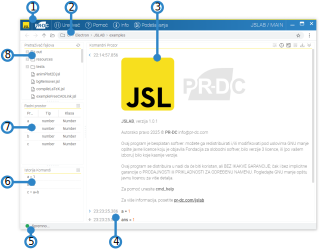
\includegraphics[width=0.8\textwidth]{resources/JSLAB_main_window.png}
    \caption{Main Window of JSLAB}
    \label{fig:main-window}
\end{figure}

Within the main window, there are various shortcuts defined in the help window---for example, the \texttt{[CTRL]} + \texttt{[H]} shortcut opens the help window.

In the image above, the following elements of the main window are numbered:
\begin{enumerate}
  \item \textbf{Main Window Header}\\
        A menu with options for opening the code editor window, viewing help, accessing program information, and opening the program settings (such as language settings; currently, Serbian in both Latin and Cyrillic scripts and English are available).
  \item \textbf{Workspace Navigation}\\
        Icons for navigating through folders and opening a folder selection window. Besides the current workspace folder, you can save additional paths that will be used when running scripts.
  \item \textbf{Command Window}\\
        Located in the central right panel, this window displays messages from the workspace after code execution.
  \item \textbf{Command Input Field}\\
        Located at the bottom of the central right panel, this field is used to send commands to the workspace. As you type, suggestions for completing the command automatically appear based on the currently active workspace. You can also navigate through the history of entered commands. After typing a command and pressing \texttt{[ENTER]}, the command is executed in the workspace.
  \item \textbf{Status Bar}\\
        A bar at the bottom of the window displaying the current state of the workspace. In the bottom left corner, an icon changes color based on that state; clicking the icon displays a tooltip with information about what is currently active in the workspace.
  \item \textbf{Command History}\\
        Located in the lower part of the left central panel, this section allows you to track the sequence of executed commands and easily re-execute a command (by double-clicking on it).
  \item \textbf{Workspace Variables}\\
        In the central part of the left panel, this area displays the name, type, and class of each active global variable created by the user in the workspace.
  \item \textbf{File Browser}\\
        Located in the upper part of the left panel, this area shows folders and files, which can be directly opened within the editor.
\end{enumerate}

\begin{quotation}
\textbf{Note:} The command window is ideal for entering a few commands. However, for more complex tasks, scripts are used.
\end{quotation}


% ----------
\subsection{Editor Window}
\label{sec:editor-window}

For \textbf{JSLAB} scripts, the \texttt{.jsl} extension is used to distinguish them from the standard \texttt{.js} extension for JavaScript. Scripts are executed by providing the script path as the sole argument to the \texttt{run} function. For writing or editing code in a script, it is best to use the built-in code editor (which can be opened with the \texttt{editor} command or the \texttt{edit()} function). The code editor window is shown in the image below.

\begin{figure}[H]
    \centering
    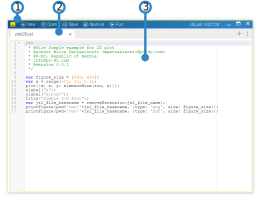
\includegraphics[width=0.8\textwidth]{resources/JSLAB_editor_window.png}
    \caption{Editor Window of JSLAB}
    \label{fig:editor-window}
\end{figure}

In the image above, the following elements of the code editor window are numbered:
\begin{enumerate}
  \item \textbf{Editor Window Header}\\
        At the very top of the window, there is a menu with options for creating new scripts, opening existing ones, saving open scripts, and directly executing scripts in the workspace.
  \item \textbf{Script Tabs}\\
        Located just below the header, these tabs allow you to switch between the active scripts being edited and to open or close scripts.
  \item \textbf{Script Text Editor}\\
        This is the area where the script code is displayed. As you type, suggestions for completing commands automatically appear based on the currently active workspace---similar to the command window. This text editor provides many advanced features for working with code, including syntax checking, suggestions, the ability to collapse certain code blocks, and highlighting of the current active line.
\end{enumerate}

The editor also includes additional advanced features for code input, such as searching through the code and performing text replacements (the search popup can be opened by pressing \texttt{[CTRL]} + \texttt{[F]}).

Most importantly, code can be executed in two ways:
\begin{itemize}
  \item By entering commands in the command input field of the command window.
  \item By running a script using the \code{run()} function or directly from the editor window.
\end{itemize}


% ----------
\subsection{Programming}
\label{sec:programming}

Programming in \textbf{JSLAB} is based on the full feature set of \textbf{JavaScript} and \textbf{Node.js}, combined with \textbf{HTML} and \textbf{CSS} for building graphical user interfaces (GUI). The application also provides a range of \textbf{built-in functions} that simplify certain tasks---like plotting with the \code{plot()} function. All implemented functions and classes are documented for easy reference.

\subsubsection{Accessing Documentation}
Multiple approaches are available to view documentation directly from \textbf{JSLAB}:
\begin{itemize}
  \item \textbf{Built-in help functions:} \code{help()}, \code{doc()}, \code{documentation()}, \code{helpSearch()}, \code{docSearch()}, \code{documentationSearch()}
  \item \textbf{HTML documentation:} Openable via the \code{openDoc()} or \code{openDocumentation()} functions
  \item \textbf{Function source code:} See the implementation of a built-in function with \code{source("functionName")} (e.g., \code{source("plot")})
\end{itemize}

\subsubsection{Working with Scripts and Examples}
\textbf{JSLAB} scripts typically use a \texttt{.jsl} extension to distinguish them from standard \texttt{.js} files. You can run scripts from the command window with \code{run("scriptPath")}, or open them in the built-in editor (using the \code{editor} command or the \code{edit("scriptName.jsl")} function).

For bundled example scripts:
\begin{itemize}
  \item \textbf{List examples:} \code{getExamples()}
  \item \textbf{Open a specific example:} \code{openExample("exampleName")}
  \item \textbf{Open the examples folder:} \code{openExamplesFolder()}
  \item \textbf{Navigate to the examples folder:} \code{goToExamplesFolder()}
\end{itemize}

\subsubsection{Resetting the Environment}
\begin{itemize}
  \item \textbf{Reset workspace (sandbox):} \code{resetSandbox()} clears current workspace variables.
  \item \textbf{Reset the entire application:} \code{resetApp()} returns the application to its initial state.
\end{itemize}

\subsubsection{Advanced Chromium Tools}
Since \textbf{JSLAB} is built on \textbf{Chromium}, you can leverage its powerful developer tools for debugging and performance analysis:
\begin{itemize}
  \item \code{openDevTools()}: Open Developer Tools
  \item \code{openWindowDevTools()}: Open Window Developer Tools
\end{itemize}

The \textbf{Performance} tab in the developer tools is particularly useful for optimizing your scripts, helping to identify potential slow-downs and bottlenecks.

% --------------------
\section{Examples}

% ----------
\subsection{Animated 2D Plot}
\label{sec:animated-2d-plot}

A 2D plot animation like this is essential for visualizing real-time data changes, enabling dynamic tracking of evolving values and providing immediate insight into trends or fluctuations as they happen.

\begin{figure}[H]
    \centering
    % If you experience issues with GIFs, consider converting to a supported format.
    \includegraphics[width=0.8\textwidth]{resources/JSLAB_2D_plot.png}
    \caption{Animated 2D Plot}
    \label{fig:animated-2d-plot}
\end{figure}

\begin{lstlisting}[style=JavaScriptStyle]
// JavaScript Example
var N_buffer = 500;
var t = toc();
var x = createFilledArray(N_buffer, null); x[0] = t;
var y = createFilledArray(N_buffer, null); y[0] = sin(t);
var p = plot({x: x, y: y});
xlabel("x");
ylabel("sin(x)");
title("Simple 2-D Plot");

await p.ready;
setInterval(function() {
  var t1 = toc();
  x.push(t1);
  y.push(sin(t1*2));
  if(x.length > N_buffer) {
    x.shift();
    y.shift();
  }
  p.update({x: [x], y: [y]}, 0);
}, 33);
\end{lstlisting}

% ----------
\subsection{3D Plot with Vectors}
\label{sec:3d-plot-vectors}

3D plots are essential for illustrating spatial relationships and complex vector interactions, allowing for a deeper understanding of data across three dimensions.

\begin{figure}[H]
    \centering
    \includegraphics[width=0.8\textwidth]{resources/JSLAB_3D_plot.png}
    \caption{3D Plot with Vectors}
    \label{fig:3d-plot-vectors}
\end{figure}

\begin{lstlisting}[style=JavaScriptStyle]
// JavaScript Example
var x = [0, 0, 0, 1, 0];
var y = [0, 0, 0, 1, 0];
var z = [0, 0, 0, 1, 0];

var u = [1, 0, 0, 1, -1];
var v = [0, 1, 0, 1, 0];
var w = [0, 0, 1, 1, 0];

var head_scale = 0.2;
var head_angleFactor = 0.4;

var vectors = createVectors3D(x, y, z, u, v, w, head_scale, head_angleFactor, {color: "#0f0", width: 6});

figure(1);
plot([
  vectors.line, vectors.head
], {'showLegend': false, 'font': {family: 'LatinModern', size: 14}});
xlabel("x");
ylabel("y");
zlabel("z");
xlim([-1, 3]);
ylim([-1, 3]);
zlim([-1, 3]);
\end{lstlisting}

% ----------
\subsection{3D Graphics}
\label{sec:3d-graphics}

3D graphics are vital for creating immersive visualizations that bring complex structures and spatial relationships to life, enabling a more intuitive understanding and interaction with digital models in fields like simulation, design, and data analysis.

\begin{figure}[H]
    \centering
    \includegraphics[width=0.8\textwidth]{resources/JSLAB_3D_graphics.png}
    \caption{3D Graphics Example}
    \label{fig:3d-graphics}
\end{figure}

\begin{lstlisting}[style=JavaScriptStyle]
// JavaScript Example
var win = await openWindow3D();
win.document.title = "Test 3D Window - JSLAB | PR-DC";
var THREE = win.THREE;

const width = win.innerWidth, height = win.innerHeight;

// init
const camera = new THREE.PerspectiveCamera( 70, width / height, 0.01, 10 );
camera.position.z = 1;

const scene = new THREE.Scene();

const geometry = new THREE.BoxGeometry( 0.2, 0.2, 0.2 );
const material = new THREE.MeshNormalMaterial();

const mesh = new THREE.Mesh( geometry, material );
scene.add( mesh );

const renderer = new THREE.WebGLRenderer( { antialias: true } );
renderer.setSize( width, height );
renderer.setAnimationLoop( animate );
win.document.body.appendChild( renderer.domElement );

// Handle window resizing
window.addEventListener('resize', onWindowResize, false);

function onWindowResize() {
  camera.aspect = win.innerWidth / win.innerHeight;
  camera.updateProjectionMatrix();
  renderer.setSize(win.innerWidth, win.innerHeight);
}

function animate( time ) {
  mesh.rotation.x = time / 2000;
  mesh.rotation.y = time / 1000;
  
  renderer.render( scene, camera );
}
\end{lstlisting}

% ----------
\subsection{Parallel Execution}
\label{sec:parallel-execution}

Parallel execution is critical for handling computationally intensive tasks, as it allows multiple operations to run simultaneously, significantly reducing processing time and improving efficiency by utilizing all available CPU cores.

\begin{lstlisting}[style=JavaScriptStyle]
// JavaScript Example
var computeSquare = (i) => i * i;

// Run parallel exectuion 
var results = await parallel.parfor(0, 20, 1, 
  parallel.getProcessorsNum(), {}, undefined, computeSquare);
disp(results);
\end{lstlisting}

% ----------
\subsection{Vector and Matrix Operations}
\label{sec:vector-matrix}

Vector and matrix operations are fundamental for efficiently performing complex mathematical computations in fields like physics, engineering, and computer graphics, enabling quick transformations, optimizations, and solutions in multidimensional spaces.

\begin{lstlisting}[style=JavaScriptStyle]
// JavaScript Example
var v1 = vec.new(1, 2, 3);
var v2 = vec.new([4, 8, 6]);
const v_cross = v1.cross(v2);

var A = mat.new([
    [1, 2],
    [3, 4]
]);
const b = mat.new([
    [5],
    [11]
]);
const x = A.linsolve(b);
disp('Solution to linear system A * x = b:');
disp(x);
\end{lstlisting}

% ----------
\subsection{Symbolic Math}
\label{sec:symbolic-math}

Symbolic math computations are essential for achieving high precision in mathematical modeling, automating algebraic simplifications, and enabling dynamic formula manipulation, which enhances the accuracy and functionality of tools in scientific, engineering, and educational software.

\begin{figure}[H]
    \centering
    \includegraphics[width=0.8\textwidth]{resources/JSLAB_symbolic.png}
    \caption{Symbolic Math Example}
    \label{fig:symbolic-math}
\end{figure}

\begin{lstlisting}[style=JavaScriptStyle]
// JavaScript Example
var le, x, E, Iz;
var p, P, invP, N, d2N;
var k_int, k_e_stretching, k_e_torsion;
var xi = range(0, 1, 0.01);

await sym.load();
[le, x, E, Iz] = sym.syms(['le', 'x', 'E', 'Iz']);

P = sym.mat([
  [1, 0, 0, 0], 
  [0, 1, 0, 0], 
  [1, le, sym.pow(le, 2), sym.pow(le, 3)], 
  [0, 1, sym.mul(2, le), sym.mul(3, sym.pow(le, 2))]
]);
p = sym.mat([[1, x, sym.pow(x, 2), sym.pow(x, 3)]]);

invP = sym.inv(P);
N = sym.mul(p, invP);
d2N = sym.diff(N, 'x', 2);

k_int = sym.mul(E, Iz, sym.intg(sym.mul(sym.transp(d2N), d2N), x, [0, le]));

Ni = sym.subs(sym.subs(N, le, 1), x, xi).toNumeric();
var N_flat = Ni.flat();

sym.showLatex(N);
sym.showLatex(k_int);
\end{lstlisting}

% ----------
\subsection{FreeCAD Link}
\label{sec:freecad-link}

Integration with FreeCAD is essential for enabling automated, precise 3D modeling workflows within applications, allowing complex geometries, structures, and engineering designs to be generated, modified, and visualized programmatically, which significantly enhances productivity in design and simulation processes.

\begin{figure}[H]
    \centering
    \includegraphics[width=0.8\textwidth]{resources/JSLAB_FreeCADLink.png}
    \caption{FreeCAD Link Example}
    \label{fig:freecad-link}
\end{figure}

\begin{lstlisting}[style=JavaScriptStyle]
// JavaScript Example
var nodes = [
  [0, 0, 0],
  [0, 10, 0],
  [10, 10, 0],
  [10, 0, 0],
  [0, 0, 10],
  [0, 10, 10],
  [10, 10, 10],
  [10, 0, 10]
];
var D = createFilledArray(nodes.length, 3);

var lines = [];
for(var i = 0; i < 4; i++) {
  var j = i+1;
  if(i == 3) {
    j = 0;
  }
  lines.push([...nodes[i], ...nodes[j]]);
  lines.push([...nodes[i+4], ...nodes[j+4]]);
  lines.push([...nodes[i], ...nodes[i+4]]);
}
var d = createFilledArray(lines.length, 1);

// Generate JSON
var nodesFile = pwd + 'out/nodes.json';
var data = {
  'Coordinates': nodes,
  'Diameters': D
};
writeFile(nodesFile, stringify(data));
var data = {
  'Coordinates': lines,
  'Diameters': d
};
beamsFile = pwd + 'out/beams.json';
writeFile(beamsFile, stringify(data));

// Run FreeCADLink 
await freecad_link.start(exe, {
  port: port,
  host: host,
  timeout: timeout,
  startup_timeout: startup_timeout
}); // Start FreeCAD program

await freecad_link.newDocument(part);
await freecad_link.callScript('MakeNodes', nodesFile, timeout);
await freecad_link.callScript('MakeBeams', beamsFile, timeout);
await freecad_link.callScript('MakeFusion', [], timeout);
await freecad_link.saveAs(model, timeout);
//await freecad_link.quit(); // Close program

deleteFile(nodesFile);
deleteFile(beamsFile);
\end{lstlisting}

% ----------
\subsection{OpenModelica Link}
\label{sec:openmodelica-link}

Integration with OpenModelica is crucial for enabling advanced simulation and analysis of complex dynamic systems directly within applications, allowing engineers to model, test, and optimize system behavior seamlessly, which enhances efficiency in design and validation processes.

\begin{lstlisting}[style=JavaScriptStyle]
// JavaScript Example
await om_link.start(exe); // Start OpenModelica program
disp(await om_link.sendExpression('getVersion()'));

disp(await om_link.sendExpression("model a end a;"));
disp(await om_link.sendExpression('loadFile("'+model+'")'));
disp(await om_link.sendExpression("getClassNames()"));
disp(await om_link.sendExpression("simulate(BouncingBall)"));
await om_link.close();
\end{lstlisting}

% --------------------
\section{Contributing}

% ----------
\subsection{Setting Up the Development Environment}

Follow the detailed \hyperref[build-instructions]{build instructions} available in this documentation.

% ----------
\subsection{Making Changes}

Follow the \hyperref[coding-style]{coding style and best practices} available in this documentation.

% ----------
\subsection{Submitting Changes}

\begin{enumerate}
    \item Create a new branch for your feature or bugfix:
\begin{verbatim}
    git checkout -b feature/your-feature-name
\end{verbatim}

    \item Make your changes and commit them with clear messages:
\begin{verbatim}
   git commit -m "Add feature X to improve Y"
\end{verbatim}

    \item Push your branch to your forked repository:
\begin{verbatim}
    git push origin feature/your-feature-name
\end{verbatim}

    \item Submit a Pull Request (PR) detailing your changes.
\end{enumerate}

% ----------
\subsection{Testing}
Before submitting a PR, ensure that all tests pass and add new tests for any new functionality you introduce.

% ----------
\subsection{Reviewing Process}
All PRs are subject to review by the maintainers. Be prepared to make revisions based on feedback to align with project standards.

% ----------
\subsection{Best Practices}

\begin{itemize}
    \item \textbf{Consistent Formatting:} Use a consistent code formatter (e.g., Prettier) to maintain uniform code style.

    \item \textbf{Meaningful Commit Messages:} Write clear and descriptive commit messages that explain the purpose of the changes.

    \item \textbf{Modular Code:} Write reusable and modular code to enhance maintainability and scalability.

    \item \textbf{Comprehensive Testing:} Implement thorough tests to ensure the reliability of your contributions.
\end{itemize}

% --------------------
\section{Feedback}

Your feedback is invaluable in improving the \textbf{JSLAB} application. Whether you encounter bugs, have feature requests, or need assistance, please reach out through the following channels:

\begin{itemize}
    \item \textbf{GitHub Issues:} Report bugs or suggest features by opening an issue in the GitHub repository.
    
    \item \textbf{Email}: Contact us directly at \href{mailto:info@pr-dc.com}{info@pr-dc.com} or main author at \href{mailto:mpetrasinovic@pr-dc.com}{mpetrasinovic@pr-dc.com}.
\end{itemize}

We encourage active participation and appreciate all forms of feedback that help us enhance the functionality and usability of \textbf{JSLAB}.

% --------------------
\section{Code references}

$JSLAB_CODE_DATA$

% ----------------------------------------
% End of document
% ----------------------------------------
\end{document}